\documentclass[12pt,oneside,a4paper]{book}
\usepackage[cm]{fullpage}
\usepackage{amsmath,amssymb,amsthm,graphicx,enumitem,float}
\usepackage{mathrsfs,dsfont}
\usepackage[utf8]{inputenc}
\usepackage[english]{babel}
\usepackage{perpage} 
\usepackage{marginnote}
\usepackage{subcaption}
\usepackage{background}
\usepackage[object=vectorian]{pgfornament} 
\usepackage{calligra}
\usepackage{tikz}
\usepackage{multirow}
\usepackage{microtype}
\graphicspath{ {./img/} }
\everymath{\displaystyle}
\usepackage{hyperref}
\usepackage{lmodern}
\hypersetup{
    colorlinks,
    citecolor=black,
    filecolor=black,
    linkcolor=blue,
    urlcolor=black
}
\MakePerPage{footnote}
\newcommand{\R}{\mathds{R}}
\newcommand{\N}{\mathds{N}}
\newcommand{\Z}{\mathds{Z}}
\newcommand{\Q}{\mathds{Q}}
\newcommand{\xn}[2]{{#1}_1{#2}\,{#1}_2{#2}\dots{#2}{#1}_n}
\newcommand{\n}[1]{1,\,2,\,\dots,#1}
\newcommand{\abs}[1]{\left\vert#1\right\vert}
\newcommand{\norm}[1]{\left\vert\left\vert#1\right\vert\right\vert}
\newcommand{\set}[1]{\left\{#1\right\}}
\newcommand{\seq}[1]{\left<#1\right>}
\newcommand{\sumnf}{\sum_{n=1}^{\infty}}

\newcommand{\newtitle}{Real Analysis II}
\newcommand{\course}{MAT311}
\newcommand{\prof}{Prof. Md Shah Noor}

\theoremstyle{remark}
\newtheorem* {rem}{Remark}
\newtheorem* {note}{Note}

\newtheorem{thm}{Theorem}[section]
\newtheorem{cor}[thm]{Corollary}
\theoremstyle{definition}
\newtheorem{prob}{Problem}[section]
\newtheorem{defn}{Definition}[section]
\newtheorem*{ex}{Example}
\newtheorem*{soln}{Solution}

\begin{document}
\begin{titlepage}
    \backgroundsetup{
        scale=1,
        opacity=1,
        angle=0,
        color=black,
        contents={
            
\begin{tikzpicture}[color=black, every node/.style={inner sep= 15pt}]
                \node (NW) [anchor=north west] at (current page.north west){\pgfornament[width=2.5cm] {61}};
                \node (NE) [anchor=north east] at (current page.north east){\pgfornament[width=2.5cm, symmetry=v]{61}};
                \node (SW) [anchor=south west] at (current page.south west){\pgfornament[width=2.5cm, symmetry=h]{61}};
                \node (SE) [anchor=south east] at (current page.south east){\pgfornament[width=2.5cm, symmetry=c]{61}};
                \foreach \i in {-4,0,4}
                \node[anchor=north,xshift=\i cm] at (current page.north){\pgfornament[scale=0.25,symmetry=v]{71}};
                \foreach \i in {-4,0,4}
                \node[xshift=\i cm, yshift=32.25 pt] at (current page.south){\pgfornament[scale=0.25,symmetry=v]{71}};
                \foreach \i in {-8,-4,0,4,8}
                \node[yshift=\i cm, xshift=32.25pt, rotate=90] at (current page.west){\pgfornament[scale=0.25,symmetry=v]{71}};
                \foreach \i in {-8,-4,0,4,8}
                \node[yshift=\i cm, xshift=-32.25pt, rotate=90] at (current page.east){\pgfornament[scale=0.25,symmetry=v]{71}};
                \foreach \i in {-11,-9,...,7,9}
                \node[anchor=west, yshift=\i cm, xshift=52.25pt, rotate=90] at (current page.west){\pgfornament[scale=0.1]{80}};
                \foreach \i in {-11,-9,...,7,9}
                \node[anchor=east, yshift=\i cm, xshift=-52.25pt, rotate=-90] at (current page.east){\pgfornament[scale=0.1]{80}};
            \end{tikzpicture}
        }
    }
\centering

\vspace*{\baselineskip}
\vspace*{75pt}

\rule{345pt}{1.6pt}\vspace*{-\baselineskip}\vspace*{2pt}
\rule{345pt}{0.4pt}

\vspace{0.6\baselineskip}

{\LARGE \calligra{\newtitle}\\} 

\vspace{0.6\baselineskip}

\rule{345pt}{0.4pt}\vspace*{-\baselineskip}\vspace{3.2pt}
\rule{345pt}{1.6pt}

\vspace{2\baselineskip}

{\scshape \Large{\course}} 

\vspace*{5\baselineskip}



\vspace{0.5\baselineskip} 

{\scshape   \Large \prof\\ }

\vspace{0.75\baselineskip} 

{\textit{\large Shahjalal University of Science and Technology}} 

\vfill 

\vspace{0.3\baselineskip} 


{\scshape \large Edited by\\  Mehedi Hasan} 
\vspace*{40pt}
\end{titlepage}
\backgroundsetup{contents={}}
\newpage
\section*{Preface}
This is a compilation of lecture notes with some books and my own thoughts. This document is not a holy text. So, if there is a mistake, solve it by your own judgement.
\pagenumbering{roman}
\newpage
\tableofcontents
\newpage
\pagenumbering{arabic}
\part{Notes}
\chapter{Metric Space}
\section{Euclidean Space}
Euclidean space or Euclidean n-space, denoted by $ \R^n $ consists of all ordered n-tuples of real numbers.\\
Symbolically, $ \R^n=\set{x\mid x=(\xn{x}{,}), \xn{x}{,}\in \R} $\\
Here the element $ x\in\R^n $ is called a point or a vector and $ \xn{x}{,} $ are called coordinates of $ x $ when $ n>1 $.\\
If $ x,y \in \R^n $ and if $ \alpha\in\R^n $ then put,\\
$ x+y=(x_1+y_1,x_2+y_2,\dots,x_n+y_n) $ and $ \alpha x=(\alpha x_1,\alpha x_2,\dots,\alpha x_n) $ so that $ x+y\in\R^n $ and $ \alpha x\in\R^n $. This defines addition and scalar multiplication of vectors. This two operations satisfy the commutative, associative and distributive laws and make $ \R^n $ into a vector space over the real field.
\begin{thm}
    $ \R^n $ with operations of addition and scalar multiplication defined previously is a vector space of dimension $ n $.
\end{thm}
\begin{defn}[Inner Product]
    The inner product (or scalar product) of $ x $ and $ y $ in $ \R^n $ is defined by $ \seq{x,y}=x\cdot y=\sum_{i=1}^{n} x_i y_i $ and the \emph{norm} or \emph{length} of a vector $ x \in \R^n $ is defined by $ \norm{x}=\seq{x,x}^{1/2}=\sum_{i=1}^{n}\left( x_i^2\right)^2  $ and the \emph{distance} between two vectors $ x $ and $ y $ of $ \R^n $ is the real number $ \text{d(x,y)}=\norm{x-y}=\left\{\sum_{i=1}^{n} \left(x_i-y_i\right)^2\right\}^{1/2} $
\end{defn}
\begin{defn}
    Let $ X $ be a metric space. All points and sets involved below are understood to be elements and subset of $ X $.
    \begin{enumerate}
        \item A \emph{neighborhood} of a point $ p\in X $ is a set $ N_\delta(p) $ containing all points $ q $ such that $ d(p,q)<\delta $. The number $ \delta $ is called the \emph{radius} of $ N_\delta(p) $. [Mathematically, $ N_\delta(p) =\set{q\mid d(p,q)<\delta}$]
        \item A point $ p $ is a \emph{limit point} (accumulation point or cluster point) of the set $ E $ if every neighborhood $ N_\delta(p) $ contains a point $ q\neq p $ such that $ q\in E $. [Mathematically, $ (N_\delta(p)-\set{p})\cap E\neq \Phi $]
        \item If $ p\in E $ and $ p $ is not a limit point of $ E $, then $ p $ is called an \emph{isolated point} of $ E $.
        \item $ E $ is \emph{closed} if every limit point of $ E $ is a point of $ E $.
        \item A point $ p $ is an \emph{interior point} of $ E $ if there is a neighborhood $ N $ of $ p $ such that $ N\subset E $
        \begin{enumerate}[label=(\roman*)]
            \item $ E $ is \emph{open} if every point of $ E $ is an interior point of $ E $.
        \end{enumerate}
        \item The \emph{complement} of $ E $, denoted by $ E^c $ is the set of all points $ p\in X $ such that $ p \notin E $
        \item $ E $ is \emph{perfect} if $ E $ is closed and every point of $ E $ is a limit point of $E $.
        \item $ E $ is \emph{bounded} if $ E $ is a real number $ M $ and a point $ q\in X $ such that $ d(p,q)<M $ for all $ p\in E $.
        \item $ E $ is \emph{dense} in $ X $ if every point of $ X $ is a limit point of $ E $, or a point of $ E $ (or both).
    \end{enumerate}
\end{defn}
\begin{note}
    The segment $ (a,b)=\set{x\in\R\mid a<x<b} $
\end{note}
\begin{note}
    In $ \R^1 $ neighborhoods are segments, whereas in $ \R^2 $ neighborhoods are interiors of circles and in $ \R^3 $ neighborhoods are interiors of spheres.
\end{note}
\begin{thm}
    Every neighborhood is an open set.
\end{thm}
\begin{proof}
    Consider the neighborhood $ E=N_r(p)=\set{q\in X\mid d(p,q)<r} $ and let $ q $ be any point of $ E $, where $ X $ is a metric space.
    \begin{figure}[H]
        \centering
        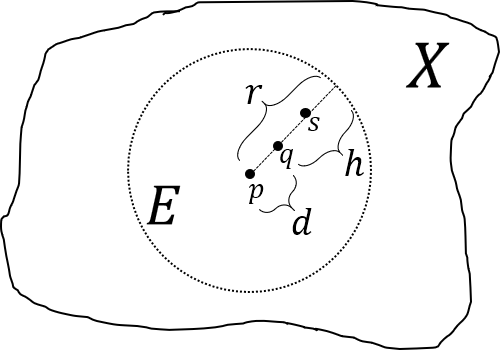
\includegraphics[scale=.75]{Picture1.png}
        % \caption{}
        \label{fig:thmNHDopen}
    \end{figure}
    Then there is a positive real number $ h $ such that $ d(p,q)=r-h $\\
    Now for all points $ s $ such that $ d(q,s)<h $,\\
    We have then\\
    \begin{tabular}{p{10cm} | l}
        $ d(p,s)\leq d(p,q)+d(q,s)<r-h+h=r $& Here $ d(p,q)<r $\\
        so that $ s\in E $ & $ \Rightarrow d(p,q)+h=r $\\
        Therefore, $ N_h(q)=\set{s\in E\mid d(q,s)<h}\subset E=N_r(p) $  & $ \Rightarrow d(p,q)=r-h $\\ 
        \cline{2-2} Thus, $ q $ is an interior point of $ E $.& $ \because r-h=d(p,q)\geq 0 $\\
        Hence the theorem. &$ \Rightarrow h\leq r $    
    \end{tabular}
    \space \qedhere
\end{proof}
\begin{thm}
    If $ p $ is a limit point of a set $ E $ in a metric space $ X $, then every neighborhood of $ p $ contains infinitely many points of $ E $.
\end{thm}
\begin{proof}
    Suppose there is a neighborhood $ N $ of $ p \in X $ which contains only a finite number of points of $ E $. Let  $\xn{q}{,} $ be those points of $ N\cap E $, which are distinct from $ p $ and put $ r=
   \operatorname*{min}_{1\leq m\leq n} d(p,q_m) $. [We use this notation to denote the smallest of the numbers $ d(p,q_1),d(p,q_2),\dots,d(p,q_n) $]\\
   The minimum of a finite set of positive numbers is clearly positive, so that $ r>0 $.\\

   The neighborhood $ N_r(p) $ contains no part $ q $ of $ E $ such that $ q\neq p $, so that $ p $ is not a limit point of $ E $.\\
   This contradiction establishes the theorem.
\end{proof}
\begin{note}
    Here $ r>0\Rightarrow r $ can be taken a large positive real number, however we please $ \Rightarrow d(p,q_m), m=1,2,\dots,n $ are bigger \& bigger $ \Rightarrow q_m $ are not close enough to $ p \Rightarrow p $ is not a limit point of $ E $. 
\end{note}
\begin{cor}
    A finite set has no limit points.
\end{cor}
\begin{prob}
    Let us consider the following subsets of $ \R^2 $
    \begin{enumerate}
        \item The set of all complex $ Z $ such that $ \abs{Z}<1 $
        \item The set of all complex $ Z $ such that $ \abs{Z}\leq1 $
        \item A finite set
        \item The set of all integers
        \item The set consisting of the numbers $ \frac{1}{n}(n=1,2,3\dots) $
        \item The set of all complex numbers (that is, $ \R^2 $)
        \item The segment $ (a,b) $
    \end{enumerate}
    If (4), (5) and (7) are regarded as subsets of $ \R^1 $, then identify whether the sets (1)-(7) are closed, open, perfect and bounded.
\end{prob}
\begin{thm}
    Let $ \set{E_\alpha} $ be a collection of sets $ E_\alpha $, then $ (\bigcup_\alpha E_\alpha)^c  = \bigcap_\alpha ({E_\alpha}^c)$
\end{thm}
\begin{thm}
    A set $ E $ is open if and only if its complement is closed.
\end{thm}
\begin{proof}
    First, suppose $ E^c $ is closed. Cause $ x\in E $. Then $ x\notin E^c $ and $ x $ is not a limit point $ E^c $. Hence there exists a neighborhood $ N $ of $ x $ such that $ E^c \cap N $ is empty, that is, $ N\subset E $. Thus $ x $ is an interior point of $ E $ and $ E $ is open.\\
    
    Next, suppose that $ E $ is open. Let $ x $ be a limit point of $ E^c $. Then every neighborhood of $ x $ contains a point of $ E^c $, such that $ x $ is not an interior point of $ E $. Since $ E $ is open, this means that $ x\in E^c $. It follows that $ E^c $ is closed.
\end{proof}
\begin{cor}
    A set $ F $ is closed if and only if its complement is open.
\end{cor}
\begin{thm}
    \begin{enumerate}
        \item For any collection $ \set{G_\alpha} $ is open sets, $ \underset{\alpha}{\cup} G_\alpha$ is open.
        \item For any collection $ \set{F_\alpha} $ is closed sets, $ \underset{\cap}{\alpha} F_\alpha$ is closed.
        \item For any finite collection $ \xn{G}{,} $ of open sets, $ \cap_{i=1}^{n} G_i $ is open.
        \item For any finite collection $ \xn{F}{,} $ of closed sets, $ \cup_{i=1}^{n} F_i $ is closed.
    \end{enumerate}
\end{thm}
\begin{note}
    Is the finiteness of the collection in parts (3) and (4) of the above theorem essential? Justify your answer.
\end{note}
\begin{defn}
    If $ X $ is a metric space, if $ E\subset X $ and if $ E' $ denotes the set of all limit points of $ E $ in $ X $, then $ E' $ is called the derived set of $ E $ and $ \bar{E}:=E\cup E' $ is called the closure of $ E $.
\end{defn}
\begin{ex}
    $ E=(0,1)\cup \set{e,\pi,\sqrt{7},11.5}, $ then $ E'=[0,1],\, \bar{E}=E'\cup E=[0,1]\cup  \set{e,\pi,\sqrt{7},11.5}$
\end{ex}
\begin{thm}
    If $ X $ is a metric space and $ E\subset X $, then 
    \begin{enumerate}[label=(\alph*)]
        \item $ \bar{E} $ is closed,
        \item $ E=\bar{E} $ if and only if $ E $ is closed,
        \item $ \bar{E}\subset F $ for every closed set $ F\subset X $ such that $ E\subset F $.
    \end{enumerate}
\end{thm}
By 1 and 3, $ \bar{E} $ is smallest closed subset of $ X $ that contains $ E $.
\begin{proof}
    \begin{enumerate}[label=(\alph*)]
        \item If $ p\in X $ and $ p\notin \bar{E} $ then $ p $ is neither a point of $ E $ nor a limit point of $ E $. Hence $ p $ has a neighborhood which does not intersect $ E $. The complement of $ \bar{E} $ is therefore open. Hence $ \bar{E}  $ is closed.
        \item If $ E=\bar{E} $, (a) implies that $ E $ is closed. If $ E $ is closed, then $ E'\subset E $(by definition (1) and (10)). Hence $ \bar{E} =E$.
        \item If $ E  $ is closed and $ F\supset E $, then $ F\supset F' $, hence $ F\supset E' $. Thus $ F\supset\bar{E} $.\\ 
        \centering\\
        \begin{tabular}{c|l}
            \multicolumn{1}{c|}{\multirow{4}{*}{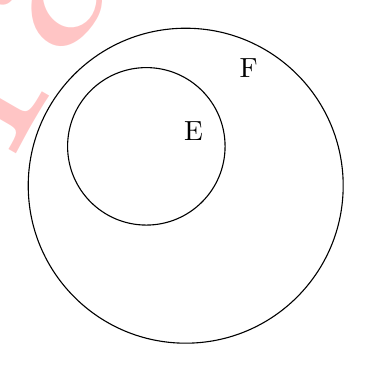
\begin{tikzpicture}
                \draw (-.5,.5) circle (1cm);
                \draw (.1,.7) node {E};
                \draw (.8,1.5) node {F};
                \draw (0,0) circle (2cm);
            \end{tikzpicture}} } &  \\
            \multicolumn{1}{c|}{} & \\ 
            \multicolumn{1}{c|}{} & $ F\supset F' $\\ 
            \multicolumn{1}{c|}{} & $ F\supset E $\\ 
            \multicolumn{1}{c|}{} & $ F\supset E' $\\
            \multicolumn{1}{c|}{} & $ F\supset \bar{E} $\\
            \multicolumn{1}{c|}{} & \\
            \multicolumn{1}{c|}{} & \\
            \end{tabular}
    \end{enumerate}
\end{proof}
\section{Connected Set}
Let $ A $ be a subset oa metric space $ X $. Two non-empty open sets $ U $ and $ V $ are said to \emph{separate} $ A $ if the satisfy these condition
\begin{enumerate}[noitemsep]
    \item $ U\cap V\cap A=\Phi $
    \item $ A\cap U\neq\Phi $
    \item $ A\cap V\neq \Phi $
    \item $ A\subset U\cup V $
\end{enumerate}
We say that $ A  $ is \emph{disconnected (i.e., not connected)} if such set exist and if such sets do not exist, we say that $ A $ is \emph{connected}.
\begin{figure}[H]
    \centering
    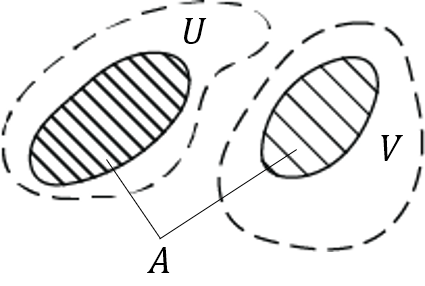
\includegraphics{Picture2.png}
    \caption{$ A $ is disconnected}
    \label{fig:conSet}
\end{figure}
\begin{ex}
    \hfill
    \begin{enumerate}
        \item $ \bar{\Z} $ is not connected
        \item $ S=\set{(x,y)\in\R^2\mid 0<x^2+y^2\leq 1} $ is connected
    \end{enumerate}
\end{ex}
\section{Compact Set}
By an open cover of a set $ E $ in a metric space $ X $ we mean a collection $ \set{G_\alpha} $ of an open subset of $ X $ such that $ E\subset \bigcup_\alpha G_\alpha $.

A subset $ K $ of a metric space $ X $ is said to be \emph{compact} if every open cover of $ K $ contains a finite subcover.

More explicitly, the requirement for completeness of $ K\subset X $ is that if $ \set{G_\alpha} $ is an open cover of $ K $, then there are finitely many indices $ \xn{\alpha}{,} $ such that
\[K\subset \xn{G_\alpha}{\cup}\quad \text{i.e.,}k\subset \bigcup_{i=1}^n {G_\alpha}_i\]
\begin{ex}
    \hfill
    \begin{enumerate}
        \item $ A=[1, 2] $ is \emph{compact}.
        \item $ B=(0, 2) $ is \emph{not compact}.
    \end{enumerate}
\end{ex}
\begin{thm}
    In a metric space, prove that closed subsets of a compact set is compact.
\end{thm}
\section{Path-connected Sets}
We say that map $ \varphi: [a,b]\to M $ of an interval $ [a,b] $ into a metric space $ M $ \emph{continuous} if $ t_\mu\to t $ implies $ \varphi(t_\mu)\to\varphi(t) $ for every sequence $ t_\mu $ in $ [a,b] $ converging to some $ t\in[a,b] $.\\

A \emph{continuous path} joining two points $ x,y $ in a metric space $ M $ is a mapping $ \varphi: [a,b]\to M $ such that $ \varphi(a)=x,\, \varphi(b)=y $ and $ \varphi $ is continuous. Here $ x $ may or may not equal $ y $ and $ b\geq a $.
\\

A path $ \varphi $ is said to lie in a set $ A $ if $ \varphi(t)\in A $ for all $ t\in [a,b] $.
\\

We say that a set $ A $ is path-connected if every two points in the set can be joined by a continuous path lying in the set.
\begin{figure}[H]
    \centering
    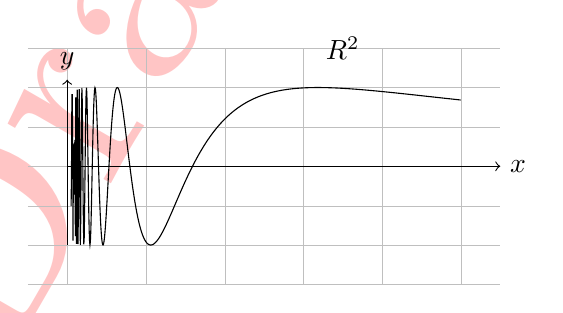
\begin{tikzpicture}[x=5cm]
        \draw[xstep=.2,ystep=.5,lightgray,ultra thin] (-0.1,-1.5) grid (1.1,1.5);
        \draw[->] (0,0) -- (1.1,0) node[right] {$x$};
        \draw[->] (0,-1) -- (0,1.1) node[above] {$y$};
        \draw (.7,1.5) node {$ \R^2 $};
        \draw[black,domain=0.01:1,samples=1000] plot (\x, {sin((1/\x)r)});
    \end{tikzpicture}
    \caption{Not path connected}
    \label{fig:path1}
\end{figure}
\begin{figure}[H]
    \centering
    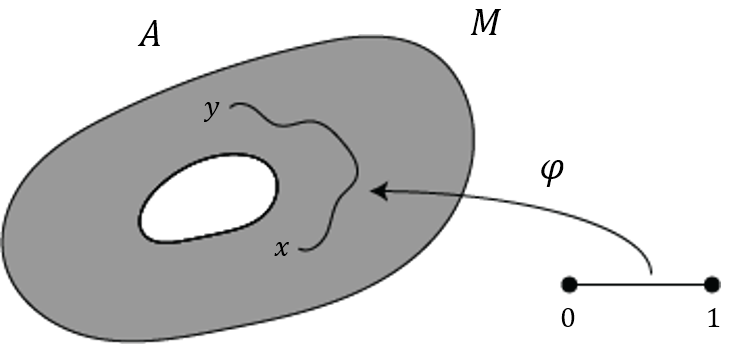
\includegraphics[scale=.5]{Picture3.png}
    \caption{Path connected}
    \label{fig:path2}
\end{figure}
\begin{itemize}
    \item Figure \ref{fig:path1}: $ A=\set{(x,\sin\frac{1}{x})\mid x>0} \cup \set{(0,y)\mid y\subset [-1,1]}\subset \R^2$. $ A $ is not path connected.\footnote{This is also known as 'Topologist's sine curve'}
    \item Figure \ref{fig:path2}: A curve joining points $ x $ and $ y $ in $ A $ of a metric space $ M $. Evidently, region $ A $ is path connected. 
\end{itemize}
\begin{prob}
    Show that $ B=[0,1] $ is path connected.
\end{prob}
\begin{soln}
    Let $ \varphi: B\to\R $ be a function defined by $ \varphi(t)=(y-x)t+x $.\\
    Here $ \varphi(0)=x $, $ \varphi(1)=y $, $ \varphi $ is continuous path (because $ \varphi $ is a linear polynomial in $ t $) and $ \varphi $ lies in $ B $.
\end{soln}
\begin{prob}
    Which of the following sets are path-connected?
    \begin{enumerate}
        \item $ [0,3] $
        \item $ [1,2] \cup [3,4 ]$
        \item $ \set{(x,y)\in\R^2\mid0<x \leq2} $
    \end{enumerate}
\end{prob}
\begin{prob}
    Let $ \varphi: B=[0,1]\to \R^2 $ be a continuous path and $ C=\varphi([0,1]) $. Show that $ C $ is path-connected.
\end{prob}
\begin{soln}
    This is intuitively clear, for we can use the path $ \varphi $ itself to join two points in $ C $. Precisely, if $ x=\varphi(a) $, $ y=\varphi(b) $, where $ 0\leq a\leq b\leq 1 $, let $ c:B\to \R^2 $ be defined by $ c(t)=\varphi(t) $. Thus $ c $ is a path joining $ x $ to $ y $ and $ c $ lies in $ C $.
\end{soln}
\begin{prob}
    Is $ \Z=\set{\dots, -2, -1, 0 ,1,2,\dots} $ connected?
\end{prob}
\begin{soln}
    No, for if $ U=(1/2, \infty) $, $ V= (-\infty,1/4) $, then $ \Z\subset U\subset V,\, \Z\cap U=\set{1,2,3,\dots}\neq \Phi    ,\, \Z\cap V=\set{\dots,-2,-1,0}\neq \Phi $. Hence $ \Z $ is not disconnected(i.e., not connected).\\
    

    Besides, $ \Z $ is not path-connected.
\end{soln}
\begin{prob}
    Are $ [0,1]\cup [2,3],\, \set{(x,y)\in\R^2\mid 0\leq x\leq1}\cup \set{(x,0)\mid 1<x<2} $ connected?
\end{prob}
\begin{prob}
    Determine the compactness of
    \begin{enumerate}
        \item finite set $ A=\set{\xn{x}{,}} $
        \item $ \R $
        \item $ B=[0,\infty) $
        \item $ C=(0,1) $
    \end{enumerate}
\end{prob}
\begin{soln}
    1. $ A=\set{\xn{x}{,}} -$ a finite subset of $ \R $.\\
    Let $ \mathscr{G}=\set{G_\alpha}  $ be any open cover of $ A $, then each $ x_i $ is contained in some set $ {G_\alpha}_i \in \mathscr{G}$. Then $ A\subset \bigcup_{i=1}^n {G_\alpha}_i \Rightarrow \set{{G_\alpha}_i ; i=1,2,\dots,n}$ is a finite sub-cover of $ \mathscr{G} $. Since $ \mathscr{G} $ is arbitrary so $ A $ is compact.
\end{soln}
\begin{thm}
    Path-connected sets are connected.
\end{thm}
\begin{thm}[Heine-Borel Theorem]
    A set $ A\subset \R^n $ is compact iff it is closed and bounded.
\end{thm}
\begin{thm}[Bolzano-Weirstrass Theorem]
    A subset of a metric space is compact iff it is sequentially compact.
\end{thm}
\begin{prob}
    Show that $ A=\set{x\in \R^n\mid \norm{x}\leq 1} $ is compact and connected.
\end{prob}
\begin{soln}
    To show that $ A $ is compact, we show it is closed and bounded. To show that it is closed consider $ A^c=\R^n\backslash A=\set{x\in \R^n\mid \norm{x}> 1}=B $. For $ x\in B,\, N_\delta(x)\subset B $, with $ \delta=\norm{x}-1 $, so that $ B $ is open and hence $ A $ is closed. It is clear that $ A $ is bounded, since $ A\subset N_2 (0) $ and therefore $ A $ is compact.\\

    To show that $ A $ is connected, we show that $ A $ is path-connected. Let $ x,y\in A $. Then the straight line joining $ x,\,y $ is the required path. Explicitly, we use $ \varphi:[0,1]\to \R^n,\,\varphi(t)=(1-t)x+ty $. One sees that $ \varphi(t)\in A $, since \begin{align*}
        \norm{\varphi(t)} &\leq\ (1-t)\norm{x}+t\norm{y}\\
        &\leq\ (1-t)+t=1\quad\text{by triangle inequality}.
    \end{align*}
\end{soln}
\begin{thm}
    Closed subsets of a compact set is compact.
\end{thm}
\begin{proof}
    Suppose $ F\subset K\subset M,\, F $ is closed subset and $ K $ is compact in the metric space $ M $. Let $ \set{V_\alpha} $ be an open cover of $ F $. If $ F^c $ is adjoined to $ \set{V_\alpha} $, we obtain an open $ \Omega $ of $ K $. Since $ K $ is compact, there is a finite sub-collection $ \Phi $ of $ \Omega $ which covers $ K $, and hence $ F $. If $ F^c $ is a member of $ \Phi $, we may remove it from $ \Phi $ and still retain an open cover of $ F $. We have thus shown that a finite sub-collection of $ \set{V_\alpha} $ covers $ F $. Hence the theorem.
\end{proof}
\chapter{Continuity}
\section{Limit}
\begin{defn}[Limit]
    Let $ X $ and $ Y $ be metric spaces; suppose $ E\subset X $, $ f $ maps $ E $ into $ Y $ (i.e., $ f:E\subset X\to Y $), and $ p $ is a limit point of $ E $. We write $ f(x)\to q $ as $ x\to p $ or $ \lim_{x\to p} f(x)=q$ if there is a point $ q\in Y $ with following property:\\
    For every $ \epsilon> 0$ there exists a $ \delta>0 $ such that $ d_Y(f(x),q)<\epsilon $ for all points $ x\in E $ for which $ 0<d_x(f(x),p)<\delta $\footnote{The $ \delta $ may depend on $ f(x),\,p, $ and $ \epsilon $ i.e., $ \delta=\delta(p,f(x),\epsilon) $} 
\end{defn}
\begin{ex}
    $ E=(0,2)\,\subset X=\R^1,\,Y=\R^1;\,f(x)=\frac{x^2-1}{x-1};\, p=1 $ is a limit point of $ E $,\\Then $ \lim_{x\to p} f(x)= \lim_{x\to 1}\frac{x^2-1}{x-1}=2$
\end{ex}
\begin{thm}[Sequential Criteron of Limits]
    Let $ x,y,E,f $ and $ p $ as in the above definition. Then $ \lim_{x\to p} f(x)=q $ iff $ \lim_{n\to \infty} f(p_n)=q $ for every sequence $ \seq{p_n} $ in $ E $ such that $ p_n\neq p $, $ \lim_{n\to \infty} p_n=p $
\end{thm}
\section{Continuity}
\begin{defn}[Continuity]
    Suppose $ X $ and $ Y $ are metric spaces, $ E\subset X,\,p\in E $ and $ f $ maps $ E \to Y (f:E\to Y) $. Then $ f $ is said to be continuous at $ p $ if for every $ \epsilon>0 $ there exists a $ \delta>0 $ such that\\
    \indent $ \mathrm{d_y(f(x), p)}<\epsilon $ for all points $ x \in E $ for which $ \mathrm{d_x(x,p)} <\delta$
\end{defn}
\begin{thm}
    Let $ f:E\subset X\to Y $ be a mapping. Then the following assertions are equivalent:
    \begin{enumerate}[label=(\roman*)]
        \item $ f $ is continuous on $ E $.
        \item For each convergent sequence $ x_n \to x_0 $, we have $ f(x_n) \to f(x_0) $
        \item For each open set $ U $ i $ Y $, $ f^{-1}(U)\subset E $ is open relative to $ E $; that is, $ f^{-1}(U)=E\cap V $ for some open set $ V $.
        \item For each closed set $ F\in Y $, $ f^{-1}(F)\subset E $ is closed relative to $ E $; that is $ f^{-1}(F)=E\cap G $ for some closed set $ G $.
    \end{enumerate}
\end{thm}
\begin{thm}
    Suppose $ f: X\to Y $ is a continuous mapping of a compact metric space $ X $ into a metric space $ Y $. Then $ f(X) $ is compact.
\end{thm}
\begin{proof}
    Let $ \set{V_\alpha} $ be an open cover of $ f(X) $, since $ f $ is continuous, by previous theorem each of the sets $ f^{-1}(V_\alpha) $ is open. Since $ X $ is compact, there are finitely many indices say $ \xn{\alpha}{,} $, such that
    \begin{equation}
        X\subset f^{-1}(V_{\alpha_1})\cup f^{-1}(V_{\alpha_2})\cup \dots\cup f^{-1}(V_{\alpha_n}) \label{eqn:cont}
    \end{equation}
    since $ f(f^{-1}(E))\subset E $ for every $ E\subset Y $, then (\ref{eqn:cont}) implies that $ f(X)\subset V_{\alpha_1}\cup V_{\alpha_2}\cup \dots \cup V_{\alpha_n} $
    This completes the proof.
\end{proof}
note to self :: There may be some page left.
\chapter{Sequences in Metric spaces}
\section{Sequences of real numbers}
A sequence of real numbers in $ \R $ is simply a function $ f:\N\to\R $ which is usually defined by $ f(n)=x_n $ and arranged in a particular order such as $ \xn{x}{,},\dots $.\\

For example, the sequence $ 1,\frac{1}{2},\frac{1}{3},\frac{1}{4},\dots $ can be represented as $ x_n=\frac{1}{n} $ for $ n=1,\,2,\,3,\dots $
\section{Convergent Sequence}
A sequence $ x_n $ in $ \R $ is said to be \emph{converge} to a \emph{limit} $ x\in \R $ if for every $ \epsilon>0 $ there is an integer $ N $ such that $ \abs{x_n-x}<\epsilon $ whenever $ n\geq N $. In this case we write $ x_n \to x $ as $ n\to \infty $ or $ \lim_{n \to \infty} x_n=x$
\begin{note}
    $ N:=N(\epsilon) $, often smaller $ \epsilon $ may require larger $ N $.
\end{note}
\section{Sequences of points or vectors in Metric Spaces}
A sequence of points in a metric space $ M:=(M,d) $ is a function $ f:\N\to M $, usually defined by $ f(n)=x_k $ and arranged in a definite order such as $ \xn{x}{,},\dots $.
\section{Convergent sequence in a Metric Space}
A sequence $ x_k $ in a metric space $ (M, d) $ converges to $ x\in M $ if for every given $ \epsilon>0 $ there is a natural number $ N $ such as $ n\geq N $ implies $ d(x_k,x_n)<\epsilon $
\section{Convergent sequence in normed space $ \R^n $} 
A sequence $ v_k $ of vectors in $ \R $ converges to the vector $ v\subset \R^n $ if for every given $ \epsilon>0 $, there exists $ N\in\N $ such that $ d(v_k,v)=\norm{v_k-v}<\epsilon $ whenever $ k\geq N $.
\section{Convergent sequence in arbitrary normed space $ V $}   
$ v_k\in V\to v\in V $ if $ \norm{v_k-v}\to 0 $ as $ k\to \infty $.\\
If $ v,v_k\in \R^n $, we write $ v=(v^1,v^2,\dots,v^n),\,v_k=(v^1_k,v^2_k,\dots,v_k^n) $
\begin{thm}
    $ v_k\to v $ in $ \R^n $ iff each sequence of coordinates converges to the corresponding coordinate of $ v $ as a sequence in $ \R $. That is,\\
    $ \lim_{k\to \infty} v_k=v$ in $ \R^n $ iff $ \lim_{k\to \infty} v_k^i=v $ in $ \R $ for each $ i=\n{n} $\\
    or,\[\lim_{k\to \infty} (v_k^1,\dots,v_k^n)= \left(\lim_{k\to \infty}v_k^1,\dots,\lim_{k\to \infty}v_k^n\right)\]
\end{thm}
\begin{ex}
    Test the convergence of the sequences in $ \R^2 $:
    \begin{enumerate}[label=(\roman*)]
        \item $ v_k=(1/k,\,1/k^2) $
        \item $ v_k=\left((\sin n)^n /n,\,1/n^2\right) $
    \end{enumerate}
\end{ex}
\begin{soln}
    \hfill
    \begin{enumerate}[label=(\roman*)]
        \item Here the component sequences $ 1/k $ and $ 1/k^2 $ each converges to 0. Hence the vectors $ v_k\to0,\, 0=(0,0)\in\R^2$
        \item Use Sandwich theorem $ \left(v_n\to (0,0)\right) $.\\
        Here, $ \abs{\frac{(\sin n)^n}{n}}=\frac{\abs{\sin n}^n}{n}\leq \frac{1}{n}\Rightarrow -\frac{1}{n}\leq \frac{(\sin n)^n}{n} \leq \frac{1}{n}$\\
        Hence by sandwich theorem, $ \lim_{n\to\infty} -\frac{(\sin n)^n}{n}=0=\lim_{n\to\infty}\frac{(\sin n)^n}{n}$, therefore,\\
        $ \lim_{n\to\infty}\frac{(\sin n)^n}{n}=0 $.\\
        Again $ \lim_{n\to\infty} \frac{1}{n^2}=0 $\\
        Therefore, $ v_n\to (0,0) $
    \end{enumerate}
\end{soln}
\begin{thm}
    A set $ A\subset M $ is closed $ \Leftrightarrow $ for every sequence $ x_k\in A $ converges to a point $ x\in A $.\label{thm:seq}
\end{thm}
\begin{ex}
    Let $ x_n \in \R^m $ be a convergent sequence with $ \norm{x_n}\leq1 $ for all $ n $. Show that the limit $ x $ also satisfies $ \norm{x}\leq1 $. If $ \norm{x_n}<1 $, then must we have $ \norm{x}<1 $? 
\end{ex}
\begin{soln}
    The unit ball $ B=\set{y\in \R^m\mid \norm{y}\leq 1} $ is closed. Let $ x_n\in B $ and $ x_n\to x \Rightarrow x\in B $ as $ B $ is closed, by theorem \ref{thm:seq}. This is not true if $ \leq $ is replaced by $ < $; for example, on $ \R $, consider $ x_n=1-\frac{1}{n} $.
\end{soln}
\section{Cauchy sequence}
Let $ (M,d) $ be a metric space. A \emph{Cauchy sequence} is a sequence $ x_k\in M $ such that for all $ \epsilon>0 $, there is an $ N\in\N $ such that $ m,n\geq N $ implies $ d(x_m,x_n)<\epsilon $.
\section{Complete Metric Space}
The metric space $ M $ is called \emph{complete} iff every Cauchy sequence in $ M $ converges to a point in $ M $.\\

In normed space, such as $ \R^n $ a sequence $ v_k $ is cauchy sequence if for every $ \epsilon>0 $ there is an $ N $ such that $ \norm{v_k-v_j}<\epsilon $ whenever $ j,k\geq N $.
\section{Bounded Sequence} 
A sequence $ x_k $ in a normed space is bounded if there is a number $ M'>0 $ such that $ \norm{x_k}\leq M $ for every $ k $.\\

In a metric space we require that there be a point $ x_0 $ such that $ d(x_k,x_0)\leq M' $ for all $ k $.
\end{document}